
\usepackage{fancyhdr}
\usepackage{lastpage}
\usepackage[utf8]{inputenc}

% Minted for syntax highliting
\usepackage{minted}
\usemintedstyle{tango}

% 
\usepackage[T1]{fontenc}
\usepackage{lmodern}

\usepackage{calc}
\usepackage{bytefield}

\usepackage{listings}
\usepackage{amsmath}

\usepackage{tikz}
\usetikzlibrary{automata,arrows,topaths,calc,positioning}
 
\usepackage{syntax}
\grammarindent=2cm


% Headers/footers styling
\pagestyle{fancy}
\fancyhf{}
\renewcommand{\headrulewidth}{0pt}

% Footer
\lfoot{ID1019}
\cfoot{KTH}
\rfoot{\thepage \hspace{1pt} / \pageref{LastPage}}

%\newcommand{\defaultpagestyle}{\thispagestyle{plain}}
\newcommand{\defaultpagestyle}{\thispagestyle{fancy}}



\title[ID1019 Ray Tracer]{A Ray Tracer}
 
 
\author{Johan Montelius}
\institute{KTH}
\date{\semester}

\begin{document}

\begin{frame}
\titlepage
\end{frame}

\begin{frame}{A programming example}

To show how to work with some Elixir programming constructs and to
discuss representation and modeling, we will implement a small ray tracer. 

\pause \vspace{20pt}

\begin{figure}
 \includegraphics[scale=0.1]{world.jpg}
\end{figure}

\end{frame}

\begin{frame}{Architecture}

modules that we will implement

\begin{itemize}
 \item {\bf vector:} vector arithmetic
 \item {\bf ray:} the description of a ray
 \item {\bf sphere:} a sphere object
 \item {\bf object:} a protocol for all objects
 \item {\bf camera:} the camera position, direction and characteristics
 \item {\bf tracer:} responsible for the tracing of rays 
 \item {\bf ppm:} how to generate a .ppm file
\end{itemize}

\pause and possibly some more

\end{frame}

\begin{frame}{ray tracing}

The basic idea of ray tracing: 

\begin{figure}
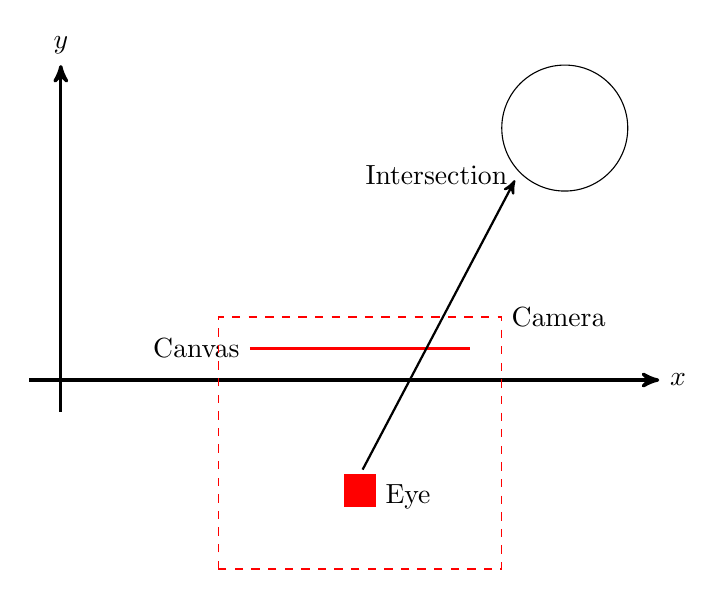
\begin{tikzpicture}[
        scale=0.4,
        axis/.style={very thick, ->, >=stealth'},
        important line/.style={thick},
        dashed line/.style={dashed, thin},
        pile/.style={thick, ->, >=stealth', shorten <=2pt, shorten >=2pt},
        every node/.style={color=black}
    ]
    % axis
    \draw[axis] (-1,0)  -- (19,0) node(xline)[right] {$x$};
    \draw[axis] (0,-1) -- (0,10) node(yline)[above] {$y$};

    \draw (16,8) circle (2);
    \pause

    \filldraw[red] (9,-4) rectangle (10,-3) node(eye)[below right]{Eye};
    \pause 
    \draw[red, thick] (6,1) node(canvas)[left] {Canvas} -- (13,1);
    \pause
    \draw[red, dashed] (5,-6) rectangle (14,2) node(camera)[right]{Camera};
    \pause
    \draw [pile] (9.5,-3) -- (14.5,6.5) node(hit)[left]{Intersection}; 
\end{tikzpicture}
\end{figure}
\end{frame}

\begin{frame}{vector arithmetic}

We first need a module to handle vector arithmetic:

\vspace{20pt}\pause

\begin{itemize}
  \pause \item Do we need to handle vectors of arbitrary dimensions?
  \pause \item How do we represent vectors?
  \pause \item What basic operations should we implement?
\end{itemize}
\end{frame}

\begin{frame}[fragile]{vector arithmetic}
\begin{columns}
 \begin{column}{0.5\linewidth}
  \begin{itemize}
   \item $a\vec{x}$ : scalar multiplication
   \item $\vec{x} - \vec{y}$ : subtraction
   \item $\vec{x} + \vec{y}$ : addition
  \end{itemize}
  \end{column}
  \pause

  \begin{column}{0.5\linewidth}
  \begin{itemize}
   \item $\|\vec{x}\|$ : norm, or length, of a vector
   \item $\vec{x} \cdot \vec{y}$ : scalar product (dot product)
   \item $|\vec{x}|$ : normalized vector $|\vec{x}| = \vec{x}/\|\vec{x}\|$
  \end{itemize}
  \end{column}
 \end{columns}

\vspace{40pt}

\pause {\em The notation for a normalized vector differ, sometimes it
  is written as $\hat{x}$}

\end{frame}


\begin{frame}[fragile]{vector arithmetic}

\begin{verbatim}
defmodule Vector do
\end{verbatim}


\begin{columns}
  \begin{column}{0.5\linewidth}
  \begin{verbatim}
def smul({x1,x2,x3}, s) do
  {x1*s, x2*s, x3*s}
end
  \end{verbatim}
\pause
  \begin{verbatim}
def add({x1,x2,x3}, {y1,y2,y3}) do
  {x1+y1, x2+y2, x3+y3}
end
  \end{verbatim}
\pause
  \begin{verbatim}
def sub({x1,x2,x3}, {y1,y2,y3}) do
  {x1-y1, x2-y2, x3-y3}
end
  \end{verbatim}
  \end{column}

  \pause

  \begin{column}{0.5\linewidth}
  \begin{verbatim}
def norm({x1,x2,x3}) do
  :math.sqrt(x1*x1 + x2*x2 + x3*x3)
end
  \end{verbatim}
  \begin{verbatim}
def dot({x1,x2,x3}, {y1,y2,y3}) do
  x1*y1 + x2*y2 + x3*y3
end
  \end{verbatim}
\pause
  \begin{verbatim}
def normalize(x) do
  n = norm(x)
  smul(x, 1 / n)
end
  \end{verbatim}
  \end{column}
 \end{columns}

\end{frame}

\begin{frame}[fragile]{objects}

We now define how to represent object and rays.

\pause
\begin{itemize}
  \item {\bf ray:} position and direction
  \item {\bf sphere:} position, radius, ...
  \item {\bf object:} a {\em protocol} for all obejcts
 \end{itemize}

\end{frame}

\begin{frame}[fragile]{rays}

  A ray is defined by an position and a direction. The position is a
  vector (a place in the space) and the direction is a {\em unit
    vector}.

\pause 

\begin{columns}[T]
 \begin{column}{0.3\linewidth}
  \begin{figure}
   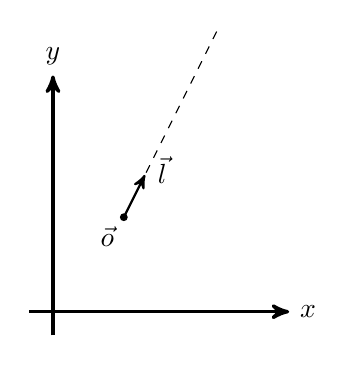
\begin{tikzpicture}[
        scale=0.3,
        axis/.style={very thick, ->, >=stealth'},
        important line/.style={thick},
        dashed line/.style={dashed, thin},
        pile/.style={thick, ->, >=stealth',  shorten >=2pt},
        every node/.style={color=black}
    ]
    % axis
    \draw[axis] (-1,0)  -- (10,0) node(xline)[right] {$x$};
    \draw[axis] (0,-1) -- (0,10) node(yline)[above] {$y$};
    \draw[fill] (3,4) node(o)[below left]{$\vec{o}$} circle (4pt);
    \draw[pile] (3,4)  -- (4,6) node()[right]{$\vec{l}$};
    \draw[dashed] (3,4) -- (7,12);
   \end{tikzpicture}
  \end{figure}  
  \end{column}

\pause

\begin{column}{0.7\linewidth}

\begin{verbatim}
defmodule Ray do

  defstruct pos: {0, 0, 0}, dir: {0, 0, 1}
\end{verbatim}

  \end{column}
 \end{columns}
\end{frame}

\begin{frame}[fragile]{tuples and structs}

 \begin{itemize}
  \item a vector: {\tt \{2, 3, 1\}}
  \item a ray:  {\tt \%Ray\{pos: \{3, 4, 0\}, dir: \{0.447, 0.894, 0\}\}}
 \end{itemize}

\pause\vspace{20pt}

\pause \vspace{10pt}
\verb+foo = %Ray{pos: {3, 2, 4}, dir: {0.447, 0.894, 0}}+

\pause \vspace{10pt}
\verb+%Ray{pos: pos} = foo+

\pause \vspace{10pt}
\verb+p = foo.pos+

\end{frame}


\begin{frame}[fragile]{Elxir protocols}

  All objects in the world should provide a function that can
  determine if it intersects with a ray.

  \pause

  Introducing protocols:
  
\begin{verbatim}
defprotocol Object do

  def intersect(object, ray)

end
\end{verbatim}

\pause\vspace{20pt}

{\em  Each object will implement the function intersect/2.}
  
\end{frame}



\begin{frame}[fragile]{spheres}

A sphere is defined by:
\vspace{20pt}\pause

\begin{columns}[T]
 \begin{column}{0.3\linewidth}
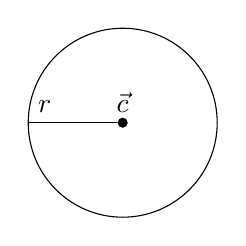
\begin{tikzpicture}[
        scale=0.4,
        important line/.style={thick},
        dashed line/.style={dashed, thin},
        pile/.style={thick, ->, >=stealth', shorten >=2pt},
        every node/.style={color=black}
    ]
    \draw (3,6) node(r)[above right]{$r$} -- (6,6);
    \draw[fill] (6,6) node()[above]{$\vec{c}$} circle (4pt);
    \draw (6,6) circle (3);
\end{tikzpicture}

 \end{column}
\pause
 \begin{column}{0.7\linewidth}
\begin{verbatim}
defmodule Sphere do

  defstruct pos: {0, 0, 0}, radius: 2

end
\end{verbatim}

 \end{column}
\end{columns}

\vspace{20pt}\pause
{\em more properties will be added later}
\end{frame}

\begin{frame}{intersection}


\begin{columns}
 \begin{column}{0.4\linewidth}
\begin{figure}
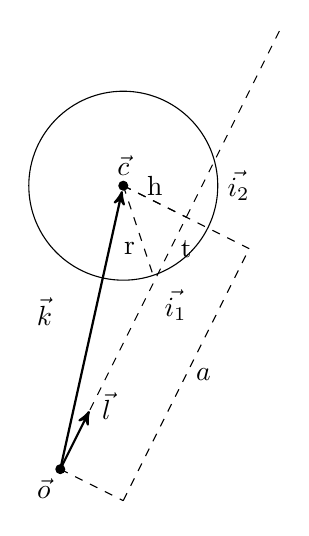
\begin{tikzpicture}[
        scale=0.4,
        important line/.style={thick},
        dashed line/.style={dashed, thin},
        pile/.style={thick, ->, >=stealth', shorten >=2pt},
        every node/.style={color=black}
    ]
    \draw[fill] (6,6) node()[above]{$\vec{c}$} circle (4pt);
    \draw (6,6) circle (3);

    \draw<2-|handout:1>[fill] (4,-3) node()[below left]{$\vec{o}$} circle (4pt);

    \draw<2-|handout:1> [dashed](4,-3) -- (11,11); 

    \draw<3-|handout:1> [thick,pile](4,-3) -- (5,-1) node(l)[right]{$\vec{l}$};  

    \draw<4-|handout:1>  (7,3) node(i1)[below right]{$\vec{i_1}$};
    \draw<4-|handout:1>  (9,6) node(i1)[right]{$\vec{i_2}$};

    \draw<5-|handout:1> [thick, pile] (4,-3) -- (6,6);
    \draw<5-|handout:1>  (3.5,2) node(k)[]{$\vec{k}$};

    \draw<7-|handout:1> [dashed] (6,6) -- (8,5);

    \draw<7-|handout:1>[dashed] (6,6) -- (10,4);  %% (4, -2)

    \draw<7-|handout:1>[dashed] (4,-3) -- (6,-4);   %% (2,-1)

    \draw<7-|handout:1>[dashed] (6,-4) -- (10,4) node()[midway, right] {$a$};

    \draw<8-|handout:1> (7,6) node()[]{h};

    \draw<10-|handout:1> [dashed] (6,6) -- (7,3);
    \draw<10-|handout:1> (6.2,4) node()[]{r};

    \draw<11-|handout:1> (8,4) node()[]{t};
\end{tikzpicture}
\end{figure}
 \end{column}
\pause 
\begin{column}{0.6\linewidth}
  \pause
  \begin{itemize}
   \uncover<6-|handout:1>{\item $\vec{k} =  \vec{c} - \vec{o}$}
   \uncover<7-|handout:1>{\item $a = \vec{l}\cdot\vec{k}$}
   \uncover<9-|handout:1>{\item $\|k\|^2 = a^2 + h^2$}
   \uncover<12-|handout:1>{\item ${r}^2 =  h^2 + t^2$}
   \uncover<13-|handout:1>{\item $ t^2 = {a}^2  - \|k\|^2   + {r}^2 $}
   \uncover<14-|handout:1>{\item $\vec{i} = \vec{o} + d \vec{l}$}
   \uncover<15-|handout:1>{\item $ d_i = a\pm t$}
   \uncover<16-|handout:1>{\item if $d_i < 0$ then $\vec{i_i}$ is {\em behind} the origin $\vec{o}$}
  \end{itemize}
 \end{column}
\end{columns} 
\end{frame}


\begin{frame}[fragile]{intersection}

\begin{columns}
 \begin{column}{0.6\linewidth}
\begin{verbatim}

defimpl Object do

 def intersect(sphere, ray) do
   k = Vector.sub(sphere.pos, ray.pos)
   a = Vector.dot(ray.dir, k)
   a2 = :math.pow(a, 2)
   k2 = :math.pow(Vector.norm(k), 2)
   r2 = :math.pow(sphere.radius, 2)
   t2 = a2 - k2 + r2
   closest(t2, a)
 end

    :

end

\end{verbatim}
 \end{column}
\pause
 \begin{column}{0.4\linewidth}
$$\vec{k} =  \vec{c} - \vec{o}$$
$$a = \vec{l}\cdot\vec{k}$$

$${t}^2 = {a}^2 - \|k\|^2 + {r}^2 $$
 \end{column}
\end{columns}
\end{frame}


\begin{frame}{ok, what else?}

\begin{figure}
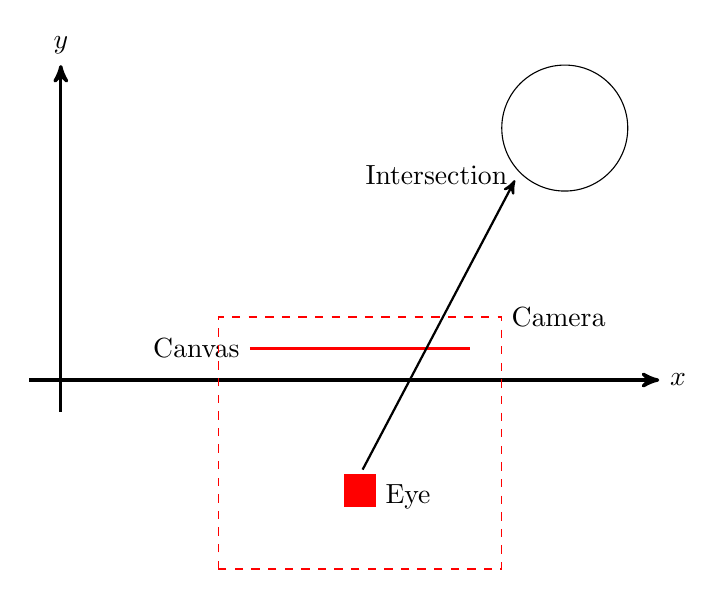
\begin{tikzpicture}[
        scale=0.4,
        axis/.style={very thick, ->, >=stealth'},
        important line/.style={thick},
        dashed line/.style={dashed, thin},
        pile/.style={thick, ->, >=stealth', shorten <=2pt, shorten >=2pt},
        every node/.style={color=black}
    ]
    % axis
    \draw[axis] (-1,0)  -- (19,0) node(xline)[right] {$x$};
    \draw[axis] (0,-1) -- (0,10) node(yline)[above] {$y$};

    \draw (16,8) circle (2);
    \pause
    \filldraw[red] (9,-4) rectangle (10,-3) node(eye)[below right]{Eye};
    \pause 
    \draw[red, thick] (6,1) node(canvas)[left] {Canvas} -- (13,1);
    \pause
    \draw[red, dashed] (5,-6) rectangle (14,2) node(camera)[right]{Camera};
    \pause
    \draw [pile] (9.5,-3) -- (14.5,6.5) node(hit)[left]{Intersection}; 
\end{tikzpicture}
\end{figure}

\end{frame}

\begin{frame}[fragile]{the camera}


\begin{columns}
 \begin{column}{0.5\linewidth}

\begin{figure}
 \includegraphics[scale=0.4]{olympusom1.jpg}
\end{figure}

 \end{column}

 \begin{column}{0.5\linewidth}
What properties do we have?
  \begin{itemize}
 \pause \item position : in space
 \pause \item direction : a unit vector 
 \pause \item size of picture : width and height
 \pause \item focal length : distance to canvas
 \pause \item resolution: pixles per distance
  \end{itemize}
 \end{column}

\end{columns}

\end{frame}

\begin{frame}[fragile]{the camera}


\begin{columns}

 \begin{column}{0.5\linewidth}

 \begin{itemize}
  \item position : in space
  \item direction : a unit vector 
  \item size of picture : width and height
  \item focal length : distance to canvas
  \item resolution: pixles per distance
  \end{itemize}
 \end{column}

 \begin{column}{0.5\linewidth}

\begin{tikzpicture}
\draw[fill] (0,0,0) node()[left]{$\vec{o}$} circle (2pt);

\draw[->] (0,0,0) -- (4,4,4) node()[below, near start]{$\vec{f}$};

\draw[->] (4,4,4) -- ++(0,2,0) node()[right, midway]{$\vec{v}$};

\draw[->] (4,4,4) -- ++(3,0,3) node()[below, midway]{$\vec{h}$};

\draw[dashed] (7,6,7) -- (7,2,7) -- (1,2,1) -- (1,6,1) -- cycle;

\end{tikzpicture}

 \end{column}
\end{columns}

\end{frame}


\begin{frame}[fragile]{the camera}


\begin{columns}

 \begin{column}{0.5\linewidth}

\begin{tikzpicture}
\draw[fill] (0,0,0) node()[left]{$\vec{o}$} circle (2pt);

\draw[->] (0,0,0) -- (4,4,4) node()[below, near start]{$\vec{f}$};

\draw[->] (4,4,4) -- ++(0,2,0) node()[right, midway]{$\vec{v}$};

\draw[->] (4,4,4) -- ++(3,0,3) node()[below, midway]{$\vec{h}$};

\draw[dashed] (7,6,7) -- (7,2,7) -- (1,2,1) -- (1,6,1) -- cycle;

\end{tikzpicture}

 \end{column}

 \pause
 \begin{column}{0.5\linewidth}

\begin{tikzpicture}
\draw[fill] (0,0,0) node()[left]{$\vec{o}$} circle (2pt);

\draw[->] (0,0,0) -- (1,6,1) node()[left, near start]{$\vec{c}$};

\draw[->] (1,6,1) -- ++(0,-1,0) node()[right, midway, anchor=east]{$\vec{d}$};

\draw[->] (1,6,1) -- ++(1,0,1) node()[above, midway, anchor=west]{$\vec{r}$};

\draw[dashed] (7,6,7) -- (7,2,7) -- (1,2,1) -- (1,6,1) -- cycle;

\end{tikzpicture}
   

 \end{column}
 
\end{columns}

\end{frame}



\begin{frame}[fragile]{a simple camera}

\begin{verbatim}
defmodule Camera do

  defstruct pos: nil, corner: nil, right: nil, down: nil, size: nil

\end{verbatim}

\end{frame}

\begin{frame}[fragile]{a normal lens pointing forward}

\begin{verbatim}
  def normal(size) do
    {width, height} = size
    d = width * 1.2
    h = width / 2
    v = height / 2
    corner = {-h, v, d}
    pos = {0, 0, 0}
    right = {1, 0, 0}
    down = {0, -1, 0}
    %Camera{pos: pos, corner: corner, .... )
  end
\end{verbatim}

\end{frame}


\begin{frame}[fragile]{rays}

Given a camera we want to find the rays from the camera ``origin'' to
the \{col,row\} position of the canvas.


\begin{columns}
 \begin{column}{0.5\linewidth}
\begin{verbatim}
def ray(camera = %Camera{}, col, row) do
  o = camera.pos
  x = Vector.smul(camera.right, col)
  y = Vector.smul(camera.down, row)
  v = Vector.add(x, y)
  p = Vector.add(camera.corner, v)
  d = Vector.normalize(p)
  %Ray{pos: o, dir: d}
end
\end{verbatim}
 \end{column}
 \begin{column}{0.5\linewidth}
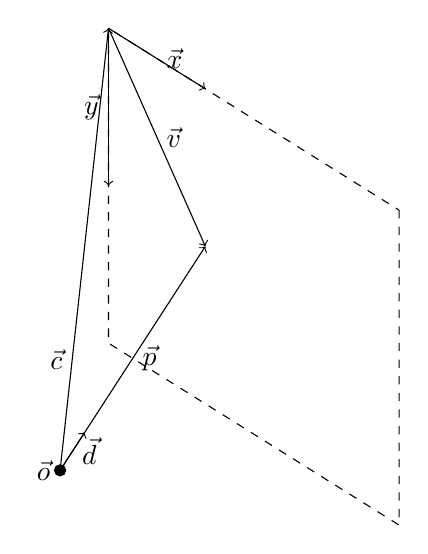
\begin{tikzpicture}
\draw[fill] (0,0,0) node()[left]{$\vec{o}$} circle (2pt);

\draw[->] (0,0,0) -- (1,6,1) node()[left, near start]{$\vec{c}$};

\draw[->] (1,6,1) -- ++(0,-2,0) node()[right, midway, anchor=east]{$\vec{y}$};

\draw[->] (1,6,1) -- ++(2,0,2) node()[above, midway, anchor=west]{$\vec{x}$};

\draw[->] (1,6,1) -- ++(2,-2,2) node()[above, midway, anchor=west]{$\vec{v}$};

\draw[->] (0,0,0) -- (3,4,3) node()[above, midway, anchor=west]{$\vec{p}$};

\draw[->] (0,0,0) -- (0.51,0.68,0.51) node()[above, midway, anchor=west]{$\vec{d}$};

\draw[dashed] (7,6,7) -- (7,2,7) -- (1,2,1) -- (1,6,1) -- cycle;

\end{tikzpicture}

 \end{column}
\end{columns}

\end{frame}


\begin{frame}{we have everything}

\begin{figure}
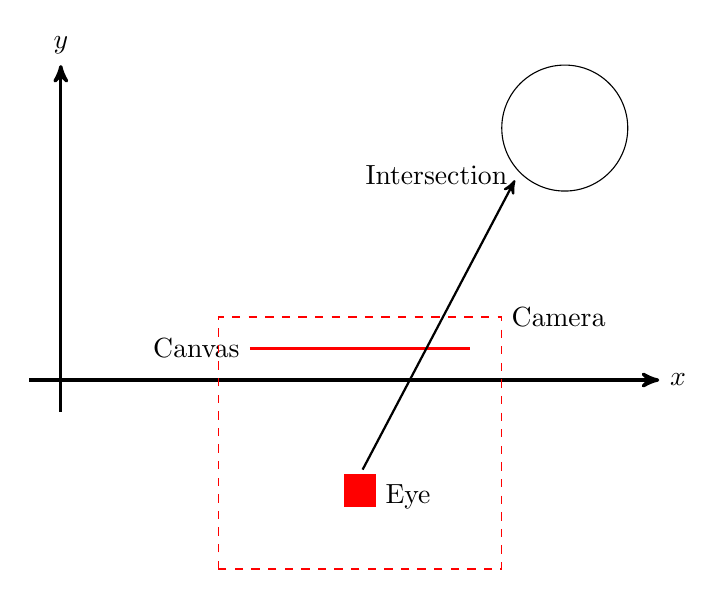
\begin{tikzpicture}[
        scale=0.4,
        axis/.style={very thick, ->, >=stealth'},
        important line/.style={thick},
        dashed line/.style={dashed, thin},
        pile/.style={thick, ->, >=stealth', shorten <=2pt, shorten >=2pt},
        every node/.style={color=black}
    ]
    % axis
    \draw[axis] (-1,0)  -- (19,0) node(xline)[right] {$x$};
    \draw[axis] (0,-1) -- (0,10) node(yline)[above] {$y$};

    \draw (16,8) circle (2);
    \pause
    \filldraw[red] (9,-4) rectangle (10,-3) node(eye)[below right]{Eye};
    \pause 
    \draw[red, thick] (6,1) node(canvas)[left] {Canvas} -- (13,1);
    \pause
    \draw[red, dashed] (5,-6) rectangle (14,2) node(camera)[right]{Camera};
    \pause
    \draw [pile] (9.5,-3) -- (14.5,6.5) node(hit)[left]{Intersection}; 
\end{tikzpicture}
\end{figure}

\end{frame}


\begin{frame}[fragile]{the tracer}

\begin{verbatim}
defmodule Tracer do

  @black {0, 0, 0}
  @white {1, 1, 1}

  def tracer(camera=%Camera{}, objects) do
    {w, h} = camera.size
    for y <- 1..h, do: for(x <- 1..w, do: trace(x, y, camera, objects))
  end

  def trace(x, y, camera, objects) do
    ray = Camera.ray(camera, x, y)
    trace(ray, objects)
  end
\end{verbatim}

\end{frame}

\begin{frame}[fragile]{tracing a ray}

\begin{verbatim}
  def trace(ray, objects) do
    case intersect(ray, objects) do
      {:inf, _} ->
        @black

      {_, _} ->
        @white
    end
  end
\end{verbatim}

\end{frame}

\begin{frame}[fragile]{the last piece}

\begin{verbatim}
  def intersect(ray, objects) do
    List.foldl(objects, {:inf, nil}, 
       fn (object, sofar) ->
            {dist, _} = sofar

            case Object.intersect(object, ray) do
              {:ok, d} when d < dist ->
                {d, object}
              _ ->
                sofar
            end
       end)
  end
\end{verbatim}

\end{frame}

\begin{frame}[fragile]{time to test}
\begin{verbatim}
defmodule Snap do

  def snap(0) do
    camera = Camera.normal({800, 600})

    obj1 = %Sphere{radius: 140, pos: {0, 0, 700}}
    obj2 = %Sphere{radius: 50, pos: {200, 0, 600}}
    obj3 = %Sphere{radius: 50, pos: {-80, 0, 400}}

    image = Tracer.tracer(camera, [obj1, obj2, obj3])
    PPM.write("snap0.ppm", image)
  end

end
\end{verbatim}
\end{frame}

\begin{frame}{snap0.ppm}

\begin{figure}
\includegraphics[scale=0.3]{snap0.png};
\end{figure}

\end{frame}


\begin{frame}[fragile]{colors}

\pause Let's add some colors to the spheres.

\begin{verbatim}
  @color {1.0, 0.4, 0.4}

  defstruct radius: 2, pos: {0, 0, 0}, color: @color 
\end{verbatim}

\pause
\begin{verbatim}
def trace(ray, objects) do
  case intersect(ray, objects) do
    {:inf, _} ->
      @black
    {_, object} ->
      object.color
  end
end
\end{verbatim}
\end{frame}


\begin{frame}{snap1.ppm}

\begin{figure}
\includegraphics[scale=0.3]{snap1.png};
\end{figure}

\end{frame}


\begin{frame}[fragile]{adding lights}

\pause We want to add some lights to the world.

\pause 
\vspace{10pt}Lights have a position and a color

\pause \vspace{10pt}The color of an intersection point is determined
by the color of the object combined with the colors from the lights.

\pause 
\vspace{10pt}Things are getting interesting.

\begin{itemize}
\item {\bf lights:} handles everything that has to do with lights and colors.
\end{itemize}

\pause \vspace{20pt}
the representation of colors is a RGB tuple of floats 0..1.0 i.e. \verb+{1.0, 0.5, 0.2}+

\end{frame}


\begin{frame}[fragile]{normal vector}


\begin{columns}
 \begin{column}{0.4\linewidth}
\begin{figure}
\begin{tikzpicture}[
        scale=0.4,
        important line/.style={thick},
        dashed line/.style={dashed, thin},
        pile/.style={thick, ->, >=stealth', shorten >=2pt},
        every node/.style={color=black}
    ]

    \draw (6,6) node(c)[above]{$\vec{c}$} circle (3);
    \draw [dashed] (4,-3) node(o)[below left]{$\vec{o}$} -- (11,11);  

    \draw [dashed] (c) -- (7.1,3.2) node(i)[]{};

    \draw (i) node[right = 0.4cm]{$\vec{i}$};

    \draw [thick, pile] (i) -- (8.19, -0.42) node(n)[right]{$\vec{n}$};
\end{tikzpicture}
\end{figure}
 \end{column}
\pause
 \begin{column}{0.6\linewidth}
$\vec{n}$ is the normal unit vector, i.e. perpendicular to the sphere, at the point of intersection.
  $$\vec{n} = |\vec{i} - \vec{c}|$$
\pause 

Will come in handy when we calculate reflection and illumination.

 \end{column}
\end{columns}

\end{frame}

\begin{frame}[fragile]{the world}

\begin{verbatim}
defmodule World do

  @background {0, 0, 0}
  @ambient {0.3, 0.3, 0.3}

  defstruct objects: [],
            lights: [],
            background: @background,
            ambient: @ambient
end
\end{verbatim}

\pause A more convenient way to handle lack of  globally accessible data structures.
 
\end{frame}

\begin{frame}[fragile]{calculating the color}

  Find all visible lights from the point of intersection; combine the
  lights \underline{give the normal vector} and illuminate the
  surface.  \pause

  In the tracer, when we have found an intersecting object:

\begin{verbatim}
 case intersect(ray, objects) do
  {:inf, _} ->
      @black
  {d, obj} ->
     o = ray.pos
     l = ray.dir
     i = Vector.add(o, Vector.smul(l, d - @delta))
     normal = Object.normal(obj,i)
     visible = visible(i, world.lights, objects)
     illumination = Light.combine(i, normal, visible)
     Light.illuminate(obj, illumination, world)
 \end{verbatim}

\end{frame}


\begin{frame}{snap2.ppm}

\begin{figure}
\includegraphics[scale=0.2]{snap2.png};
\end{figure}

\end{frame}

\begin{frame}{the fun part}

The color of an intersection point depends on:

\begin{itemize}
 \pause \item color of the object
 \pause \item combination of light sources 
 \pause \item reflection from other objects
\end{itemize}

\end{frame}


\begin{frame}[fragile]{the recursive call}

\pause 
\begin{verbatim}
  defp trace(_ray, 0, world) do
    world.background
  end

  defp trace(ray, depth, world) do
    objects = world.objects

        :
        :
      reflection = trace(r, depth - 1, world)
      Light.illuminate(obj, reflection, illumination, world)
    end
  end

\end{verbatim}

\end{frame}

\begin{frame}{snap3.ppm}

\begin{figure}
\includegraphics[scale=0.2]{snap3.png};
\end{figure}

\end{frame}


\begin{frame}{what more}

This was only scratching the surface of ray tracing.

\end{frame}

\begin{frame}{from an architecture point of view}

\begin{itemize}
 \pause \item divide program into areas of responsibility
 \pause \item think about abstractions
 \pause \item modules are similar to class definitions
 \pause \item a static type system would have helped us (structa are only halfway)
\end{itemize}

\end{frame}

\end{document}
